\documentclass[11pt]{article}
\usepackage{hyperref} 
\usepackage{amsmath, amsfonts, amssymb}
\usepackage{graphicx}
\usepackage{float}
\usepackage[margin=1in]{geometry}

\parindent0px

\emergencystretch=0pt
\pretolerance=150
\tolerance=10000
\hbadness=10000
\hfuzz=0pt

\title{Time Series Notes}
\author{Nathan Ueda}
\date{\today} 

\begin{document}
\maketitle 
\pagebreak
\tableofcontents 
\pagebreak

\section{Time Series Basics}
% \subsection{The History of Probability}

\textbf{What is a time series?}
\begin{itemize}
    \item A \textit{time series} is a sequence of observations of the same variable indexed in 
    time order (i.e. monthly stock returns). 
    \item Defining $x_t$ as a r.v., a time series may be written 
    \[ \{x_1, x_2, \ldots, x_T\} \text{ or }  \{x_t\}, \, t = 1, 2, \ldots, T \]
\end{itemize}


\textbf{Common time series properties}
\begin{itemize}
    \item Time series are typically not i.i.d. (i.e. if GNP is unusually high today, GNP will 
    likely be unusually high tomorrow).
\end{itemize}

\textbf{Modeling time series data}
\begin{itemize}
    \item The models impose structure, so when dealing with model selection, it is important 
    to evaluate to see if the model captures the features you believe to be present in the data.
\end{itemize}

\section{Stationarity}
\subsection{Strongly Stationarity and Weakly Stationarity}
\begin{itemize}
    \item A process $\{x_t\}$ is \textit{strongly stationary} or \textit{strictly stationary}
    if all aspects of its behavior are unchanged by shifts in time. More formally, it is
    defined as the requirement that for every $m$ and $n$, the distributions of $\{x_1, \ldots,
    x_n\}$ and $\{x_{1+m}, \ldots, x_{n+m}\}$ are the same, that is, the probability 
    distribution of a sequence of $n$ observations does not depend on their time origin.
   \item A process $\{x_t\}$ is \textit{weakly stationary} or \textit{covariance stationary} if 
   its mean, variance, and covariance are unchanged by time shifts. More formally, it is 
   defined as weakly stationary if 
   \begin{itemize}
    \item First moment is a finite constant: $E(x_t) = \mu$
    \item Second moment is a finite constant: $Var(x_t) = \sigma^2$
    \item $\text{Cov}(x_t, x_s) - \gamma(|t-s|)$
   \end{itemize}
   In other words, the mean and variance do not change with time and the covariance between 
   two observations depends on the time distance between them (aka having same number of 
   observations), not the specific points. 
   \item Strong stationarity does not imply weak stationarity and weak stationarity does not 
   imply strong stationarity.    
   \item Stationarity is important as a stationary process can be modeled with relatively few 
   paramters.
\end{itemize}

\subsection{Testing for Stationarity}
\begin{itemize}
    \item When a times series is observed, a natural question is whether it appears to be 
    stationary. 
    
    \item \textbf{Time series plot}:
    Looking at a \textit{time series plot} (plot of the series in chronological 
    order) may be useful. If the time series is a stationary series, it should show some random 
    oscillation around some fixed level, a phenomenon called \textit{mean reversion}. If the 
    series wanders without returning repeatedly to some fixed level, then the series should not
    be modeled as a stationary process. 
 
    \begin{figure}[H] 
         \centering 
         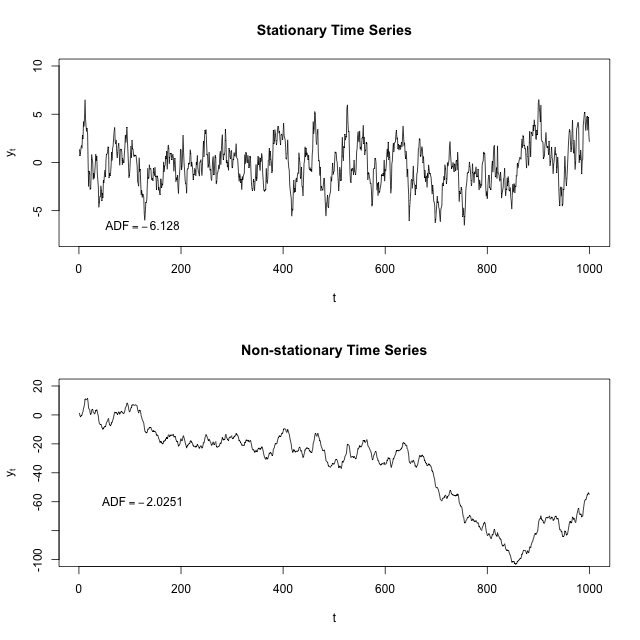
\includegraphics[width=4in]{imgs/stationary_vs_nonstationary.png}
         \caption{Stationary vs. non-stationary time series}
     \end{figure}
\end{itemize}

\section{White Noise}

\begin{figure}[H] 
    \centering 
    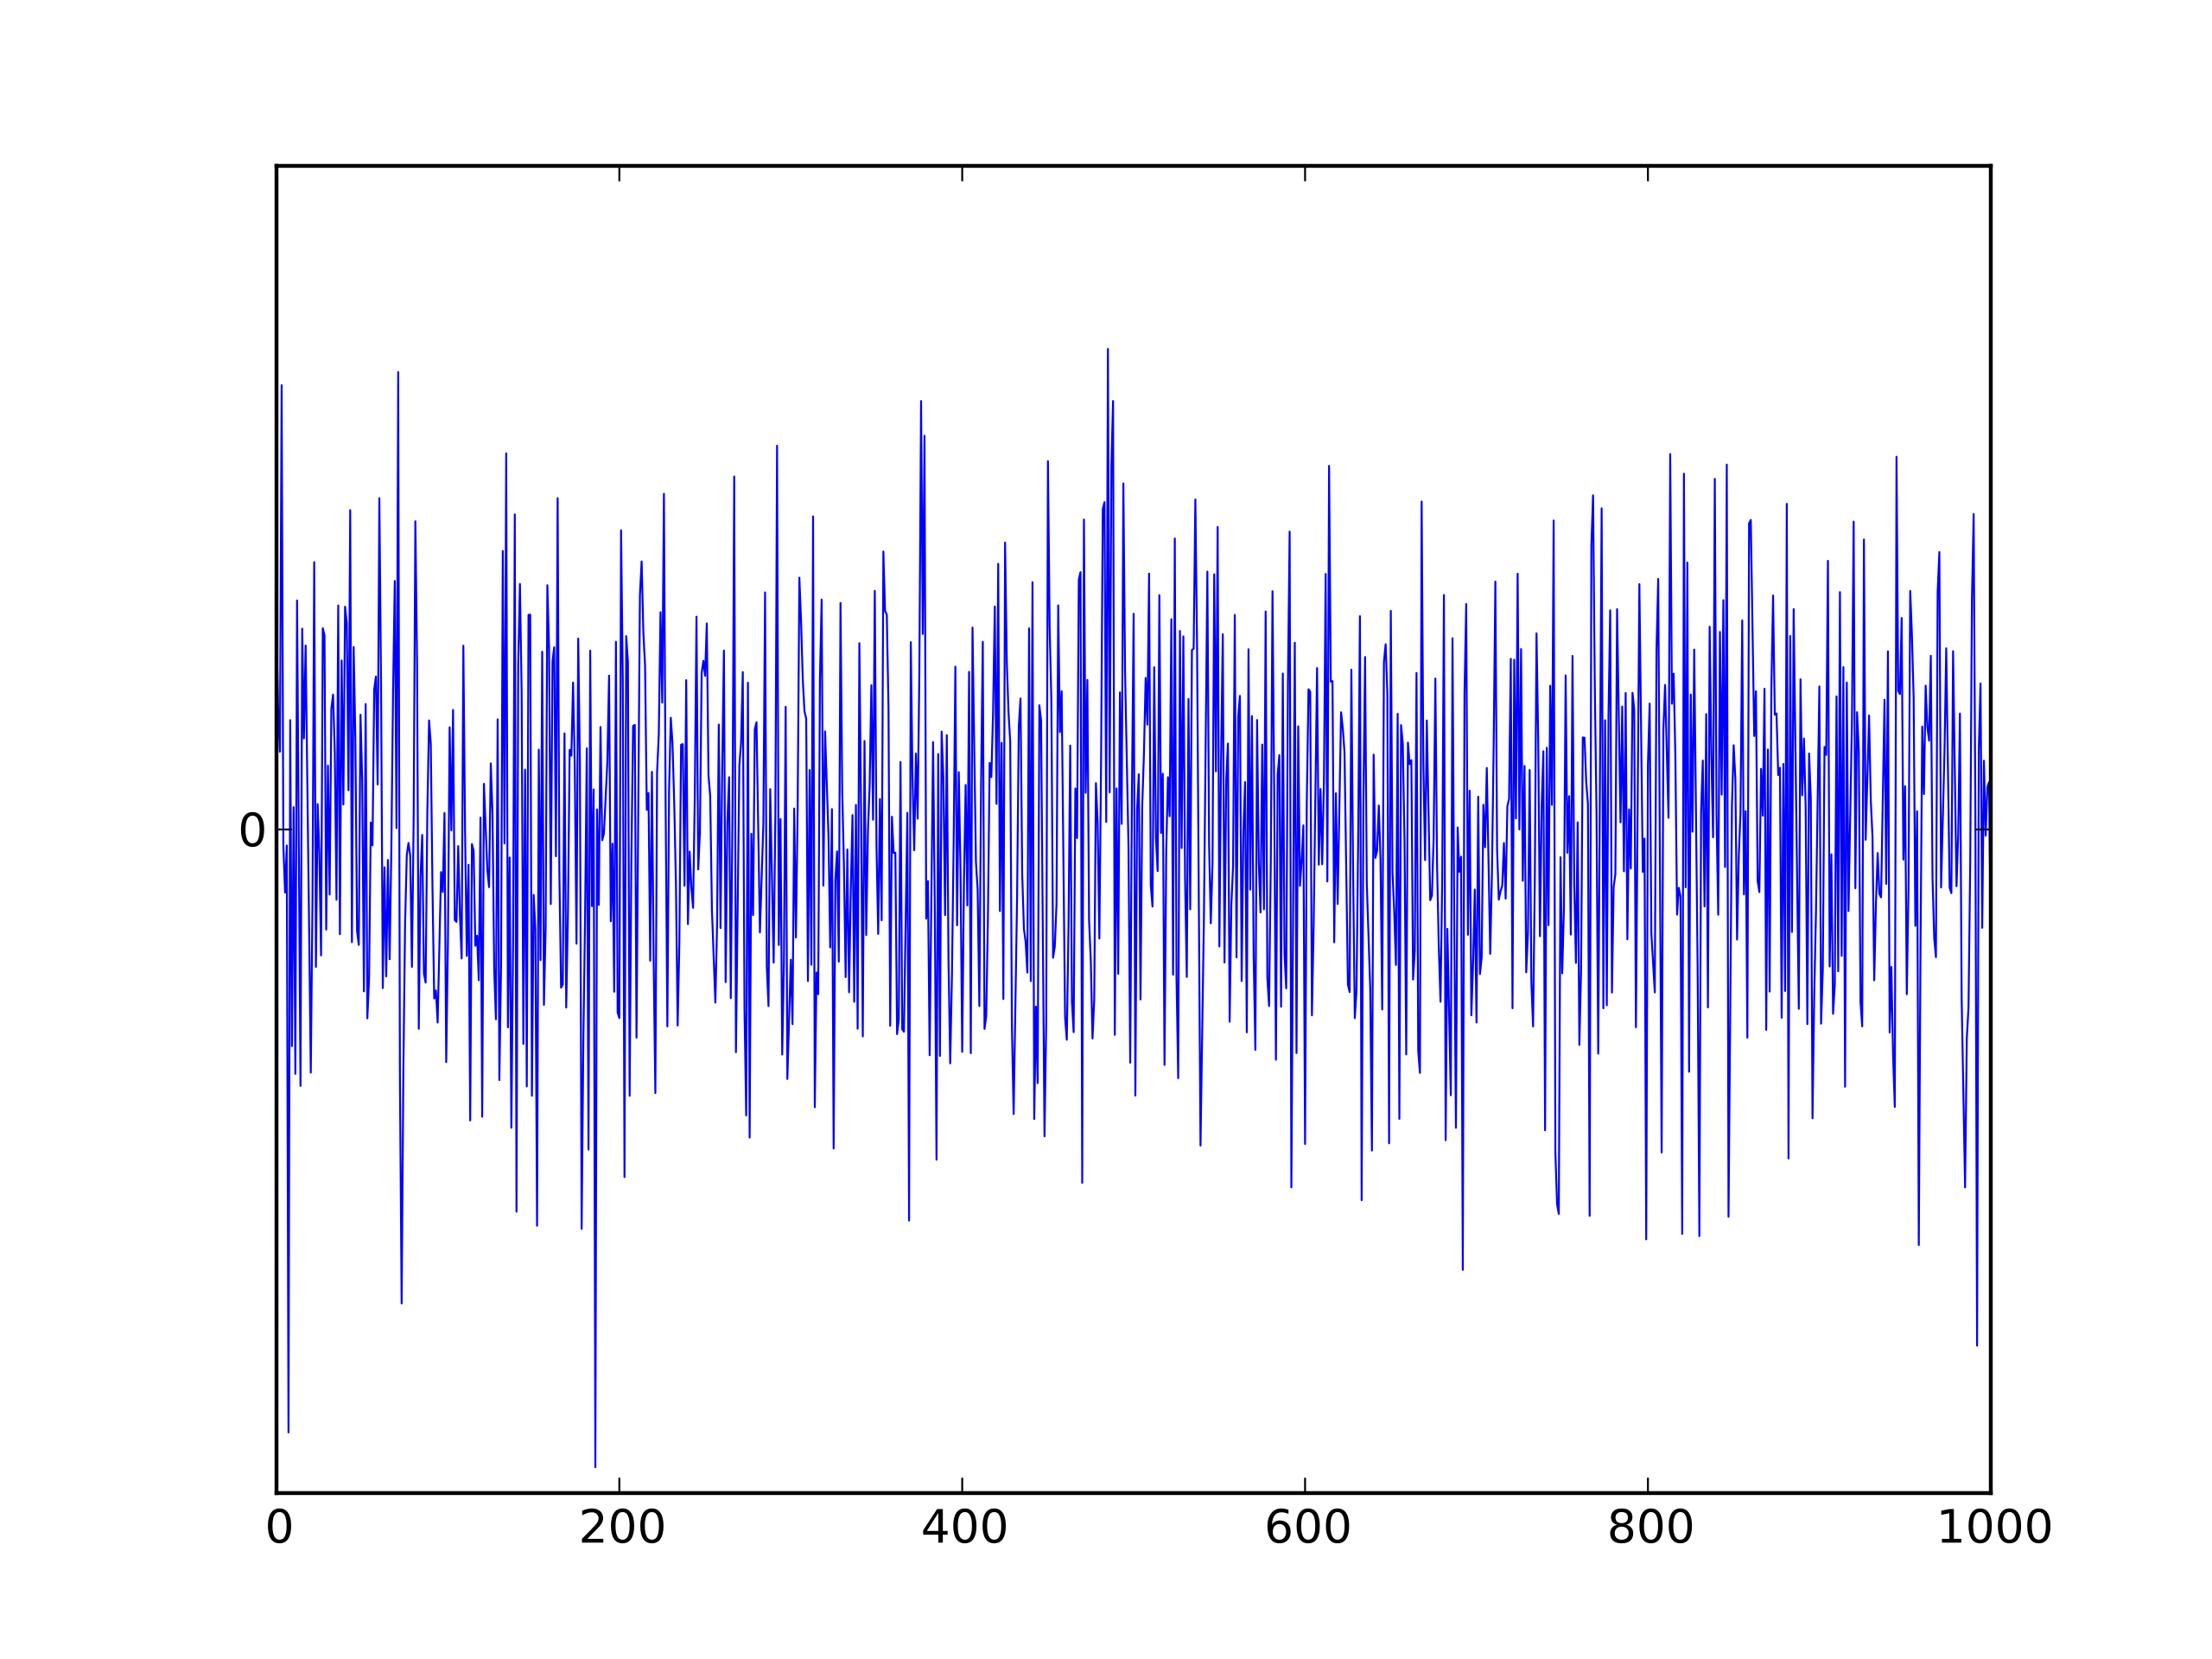
\includegraphics[width=4in]{imgs/white_noise.png}
    \caption{White noise}
\end{figure}

\begin{itemize}
    \item The building block for time series models is the \textit{white noise process}, 
    denoted $\epsilon_t$.
    \item In the least general case,
    \[ \epsilon_t \sim \text{i.i.d. } N(0, \sigma_{\epsilon}^{2})\]
    The assumption of i.i.d. have the following implications 
    \begin{enumerate}
        \item No predictability: Past values of a white noise process contain no information to predict future 
        values. Therefore, the best predictor is its mean, which is the same prediction without 
        observing past values. More formally, 
        \[E(\epsilon) = E(\epsilon_t | \epsilon_{t-1}, \epsilon_{t-2} \ldots) = 0\]
        \item No autocorrelation: Each observation is independent each other. More formally, 
        \[E(\epsilon_t \epsilon_{t-j}) = \text{Cov}(\epsilon_t \epsilon_{t-j})=0\]
        \item Conditional homoskedasticity: The conditional variance is a constant, and is 
        the same variance without observing past values. More formally, 
        \[\text{Var}(\epsilon_t) = \text{ Var}(\epsilon_t | \epsilon_{t-1}, \epsilon_{t-2} 
        \ldots) = \sigma_{\epsilon}^{2}\]
    \end{enumerate}
\end{itemize}

\section{Autocovariance and Autocorrelation}

\subsection{Autocovariance}
\begin{itemize}
    \item Autocovariance: Specifies the covariance between the value of a process at two times.
    \item Covariance: A nonstandardized measure to quantify the relationship between two 
    variables. Can take on any value. A positive value means the variables tend to move in the 
    same direction, a negative values means the variables tend to move in the opposite 
    direction, and a zero value means they are independent and don't move in relation to each 
    other.
    \item The \textit{autocovariance} of a series $x_t$ is defined as 
    \[\gamma_j = \text{Cov}(x_t, x_{t-j})\]
    \item $\gamma(h) = \gamma(-h)$ since what is important is the the space between the two 
    observations, rather than the exact observations themselves. 
    \item $\gamma_0 = \sigma^2$
\end{itemize}

\subsection{Autocorrelation}
\begin{itemize}
    \item Autocorrelation (serial correlation): The degree of correlation of the same variable 
    between different time intervals.
    \item Correlation: A standardized measure to quantify the relationship between two 
    variables. Can take on a value inclusively between -1 and 1.
    \item A time series with autocorrleation implies that, predictive power (i.e. knowing the
    price of a stock today helps forecast its price tomorrow).
    \item The \textit{autocorrelation} of a series $x_t$ is defined as 
    \[\rho_j = \frac{\gamma_j}{\gamma_0}\]
\end{itemize}

\subsection{Testing for autocorrelation}
\textbf{ACF Plots}
\begin{itemize}
    \item Show a correlation between a time series and lagged versions of itself. 
    \item The plot also includes test bounds used to test the null hypothesis that an 
    autocorrelation coefficient is 0. The null is rejected if the sample autocorrelatioon is
    outside the bounds, The usual level of the test is 0.05, so one can expect to see about 1
    out of 20 samples outside the bounds simply by chance. 

    \begin{figure}[H] 
        \centering 
        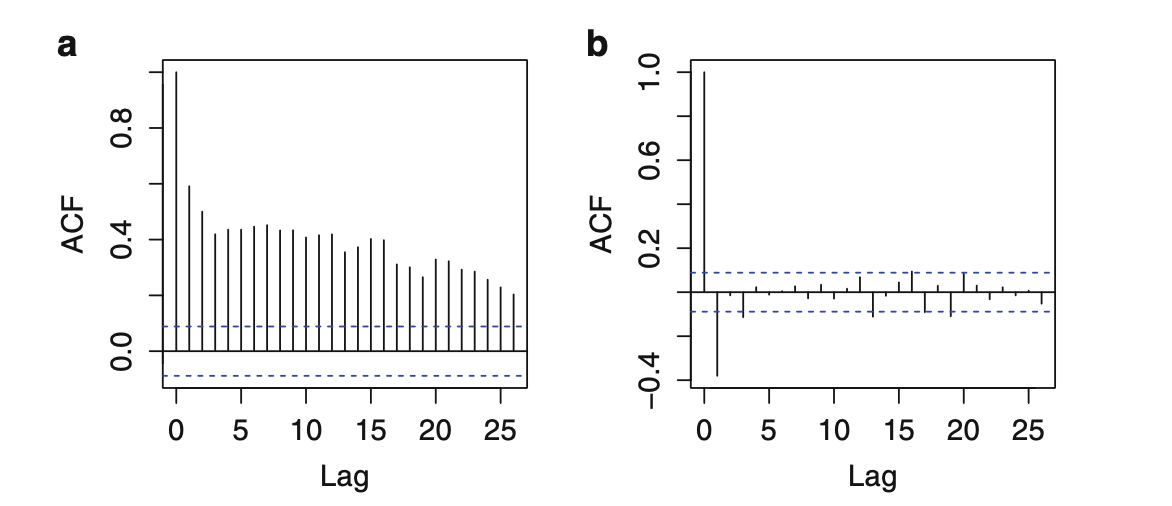
\includegraphics[width=5in]{imgs/acf_plots.png}
        \caption{Sample ACF plots of (a) one-month inflation rate (decays slowly, indicating 
        either nonstationarity or long-memory dependence) and (b) changes in the inflation rate
        (decays to 0 quickly, indicating that it is stationary).}
    \end{figure}

\end{itemize}

\textbf{Ljung-Box Test}
\begin{itemize}
    \item A \textit{simultaneous test} is one that tests whether a group of null hypotheses area
    all true versus the alternative that at least one of them is false.
    \item The \textit{Ljung-Box test} is a simultaneous test where the null is $\rho_1 = \rho_2
    = \hdots =\rho_K$ for some $K$. 
    \item If the Ljung-Box test rejects, then we conclude that one or more of $\rho_1, \rho_2, 
    \ldots, \rho_K$ is nonzero. 
\end{itemize}

\section{Autoregressive Processes}

\begin{itemize}
    \item Time series models with correlation can be constructed from white noise.
    \item The simplest correlated stationary processess are \textit{autoregressive processeses},
    where $\{x_t\}$ is modeled as a weighted average of past observations plus a white noise 
    ``error.''
    \item The term \textit{autoregression} refers to the regression of the process on its own 
    past values. 
\end{itemize}

\subsection{AR(1) Models}
\begin{itemize}
    \item Let $\epsilon_1, \epsilon_2, \ldots$ be $\text{WN}(0, \sigma_{\epsilon}^{2})$. Then 
    $\{x_t\}$ is an $\text{AR}(1)$ process if, for some constant parameter $\phi$
    \[ x_t = \phi x_{t-1} + \epsilon_t \]
    for all $t$.
    \item $\phi x_{t-1}$ may be thought of as representing the memory of the past observation
    into the present value of the process. This is what we believe we can model and predict.
    \item $\phi$ determines the amount of feedback, where a larger absolute value results in 
    more feedback.
    \item $\epsilon_t$ represents the effect of new information that cannot be modeled, hence,
    it is represented as white noise. This is what we cannot model nor predict. 
    \item Properties of a Stationary AR(1) Process 
    \begin{itemize}
        \item $E(x_t) = \mu$ 
        \item $\text{Var}(x_t)= \gamma_0 = \sigma_x^2 = \frac{\sigma_{\epsilon_t}^{2}}{1-\
        phi^2}$
    \end{itemize}
    \item The ACF of an AR(1) process depends only on one parameter, $\phi$. This parsimony 
    comes at the cost that the ACF has only a very limited range of shapes. If the ACF does not
    behave in one of these shapes, the AR(1) model is not suitable.
    \begin{figure}[H] 
        \centering 
        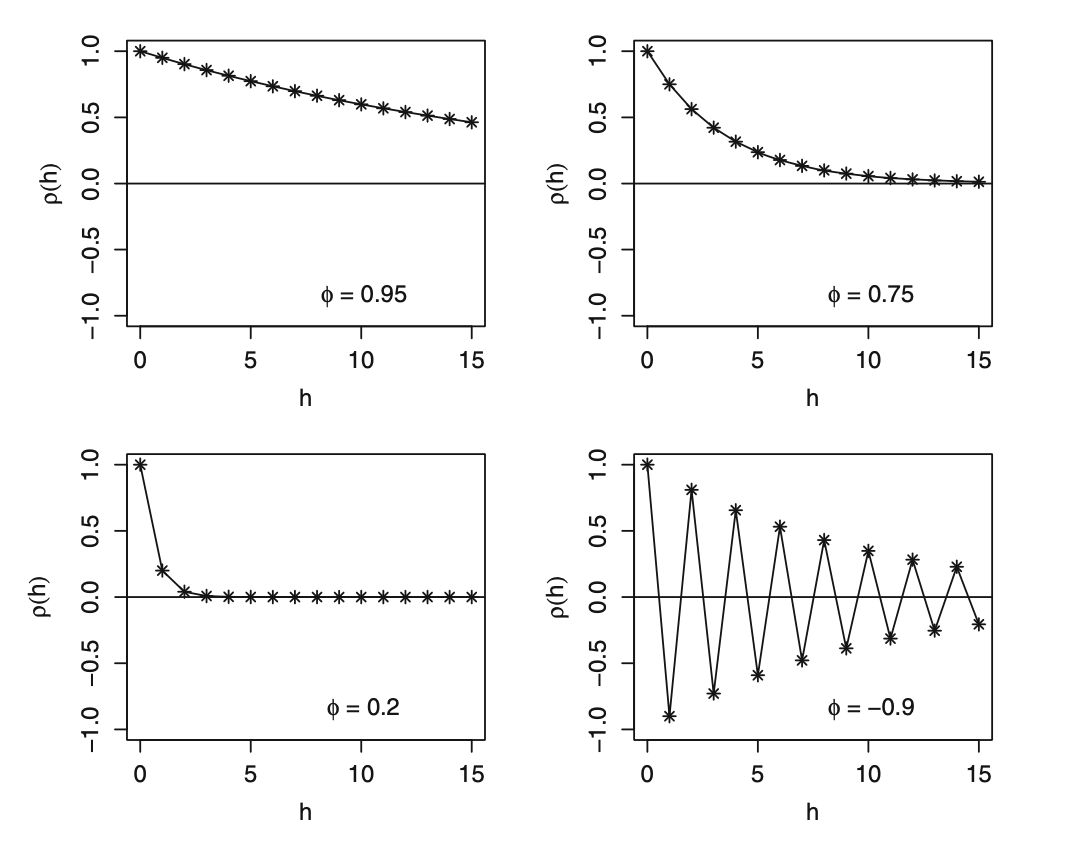
\includegraphics[width=5in]{imgs/ar1_acf.png}
        \caption{ACF of AR(1) processes with $\phi$ equal to 0.95, 0.75, 0.2, and -0.9.}
    \end{figure}
    \item When $|\phi| < 1$ the process is stationary.
    \item When $\phi=1$ the process is not stationary and takes the form of a random walk.
    Recall a random walk, in each period, takes a step random step that is i.i.d. from its 
    previous steps. 
    \item When $|\phi|>1$ the process is non-stationary and has explosive behavior.
    \item A non-zero value of $\phi$ mean that there is some information in the previous
    observation, but a small value of $\phi$ means the prediction will not be very accurate.
\end{itemize}

\subsection{AR($p$) Models}
\begin{itemize}
    \item A more flexible adaptation of an AR model that is still parsimonious and regresses on
    the $p$ past values.
    \item Let $\epsilon_1, \epsilon_2, \ldots$ be $\text{WN}(0, \sigma_{\epsilon}^{2})$. Then 
    $\{x_t\}$ is an $\text{AR}(p)$ process if, for constant parameters $\phi_1, \phi_2, \hdots,
    \phi_{t-p}$
    \[x_t = \phi_1 x_{t-1} + \phi_2 x_{t-2} + \hdots + \phi_p x_{t-p} + \epsilon_t\]
    \item If the $\text{AR}(p)$ model fits the time series well, then the residuals should look 
    like white noise. The residual autocorrelation can be detected examining the sample ACF of
    the residuals and using the Ljung-Box test. Any significant residual autocorrelation is a sign 
    the $\text{AR}(p)$ model does not fit well.
    \item A problem with AR models is that they often need a rather large value of $p$ to fit 
    a dataset.
    %%%%%% YULE WALKER?
\end{itemize}

\section{Moving Average Processes}


\section{Misc.}
\begin{itemize}
    \item Returns are closer to i.i.d. than prices and overall exhibit more attractive 
    statistical qualities than prices, therefore making it more sensible to study returns 
    rather than prices. 
\end{itemize}

\section{Definitions}
\begin{itemize}
    \item Homoskedasticity: A condition in which the variance of the residual is constant, that
    is, the error term does not vary much. In other words, the variance of the data points is 
    roughly the same for all data points. 
\end{itemize}

\end{document}
